\section{Grafici e immagini}

\begin{figure}[h]
	\centering
	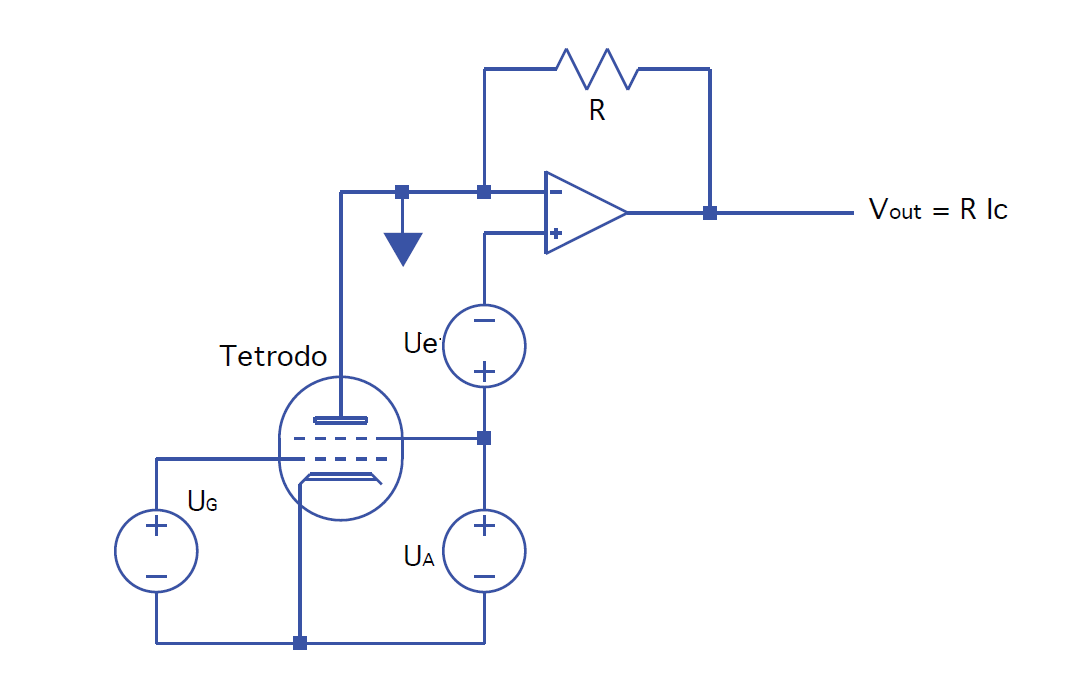
\includegraphics[scale=0.5]{apparato.png}
	\caption{Apparato usato nell'esperienza.}
	\label{f:apparato}
\end{figure}
\begin{figure}[h]
	\centering
	\includegraphics[scale=0.6]{foto_32.JPG}
	\caption{V$_{heat} = 4$ V}
	\label{f:figura_3}
\end{figure}
\begin{figure}[h]
	\centering
	\includegraphics[scale=0.7]{foto_33.JPG}
	\caption{V$_{heat} = 5$ V}
           \label{f:figura_4}
\end{figure}
\begin{figure}[h]
	\centering
	\includegraphics[scale=0.6]{foto_34.JPG}
	\caption{V$_{heat} = 6$ V}
	\label{f:figura_5}
\end{figure}
\begin{figure}[h]
	\centering
	\includegraphics[scale=0.7]{foto_35.JPG}
	\caption{V$_{heat} = 7$ V.}
           \label{f:figura_6}
\end{figure}
\begin{figure}[h]
	\centering
	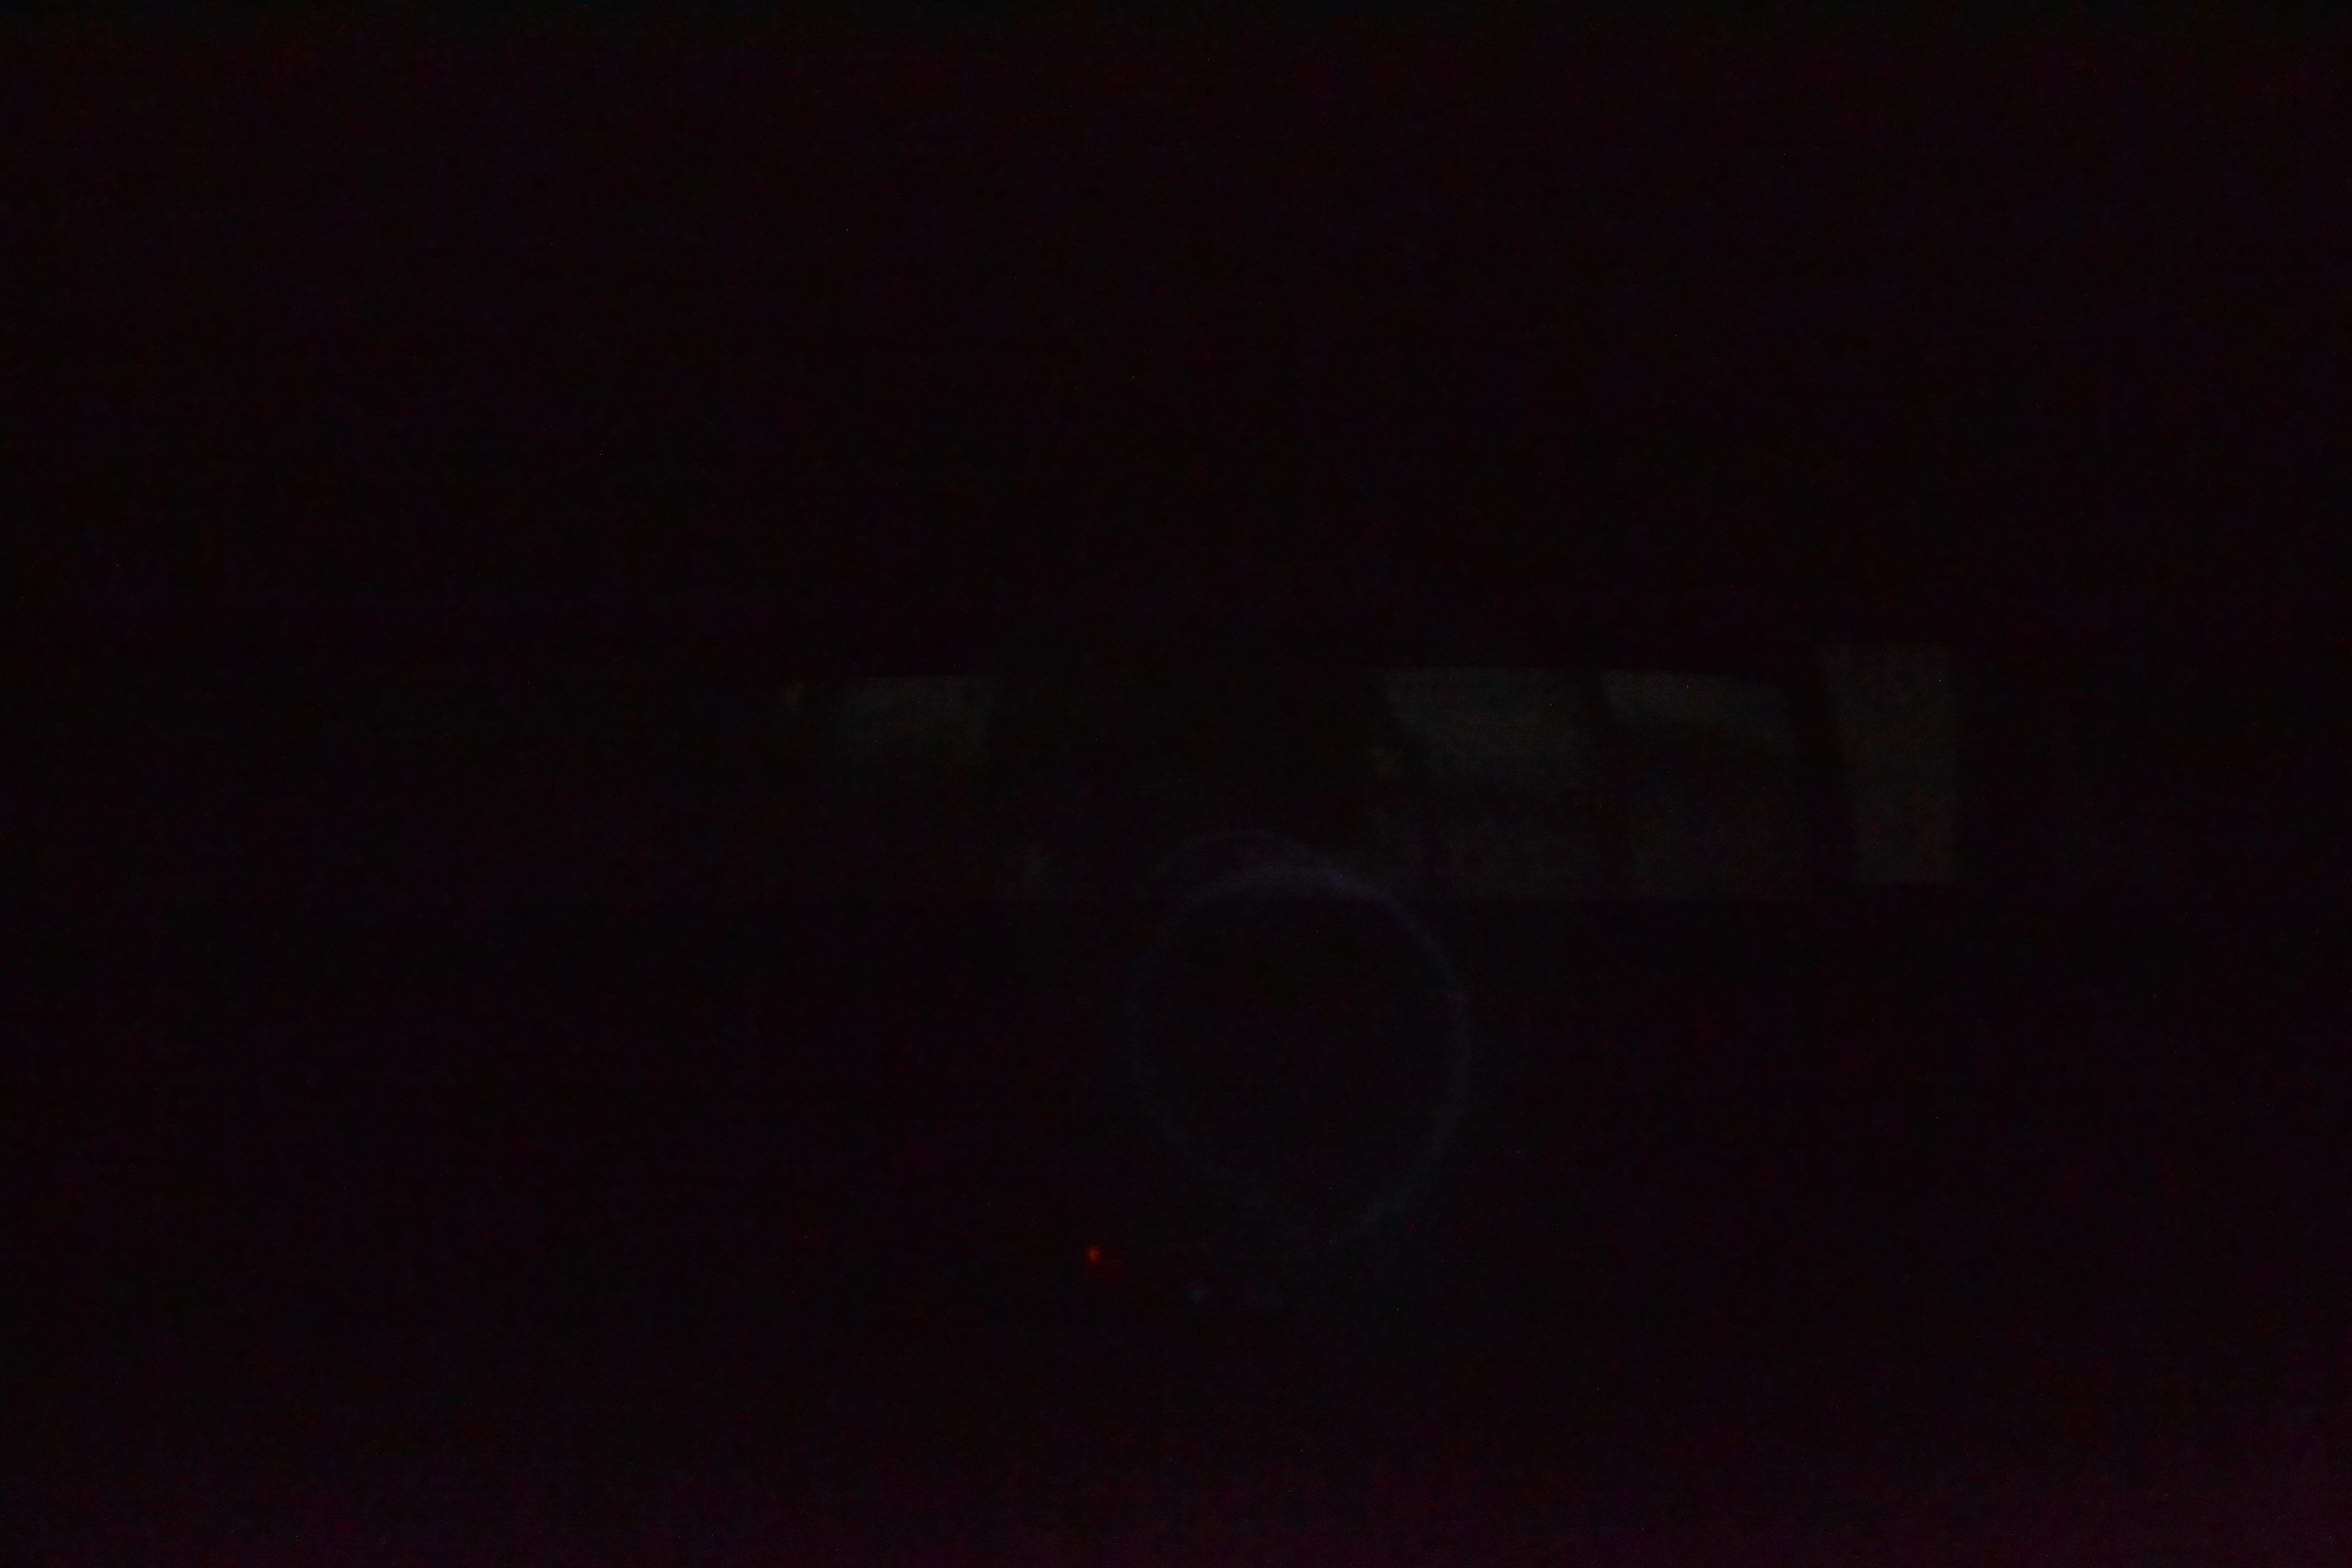
\includegraphics[scale=0.7]{foto_36.JPG}
	\caption{V$_{heat} = 3$ V.}
           \label{f:figura_7}
\end{figure}
\begin{figure}[h]
	\centering
	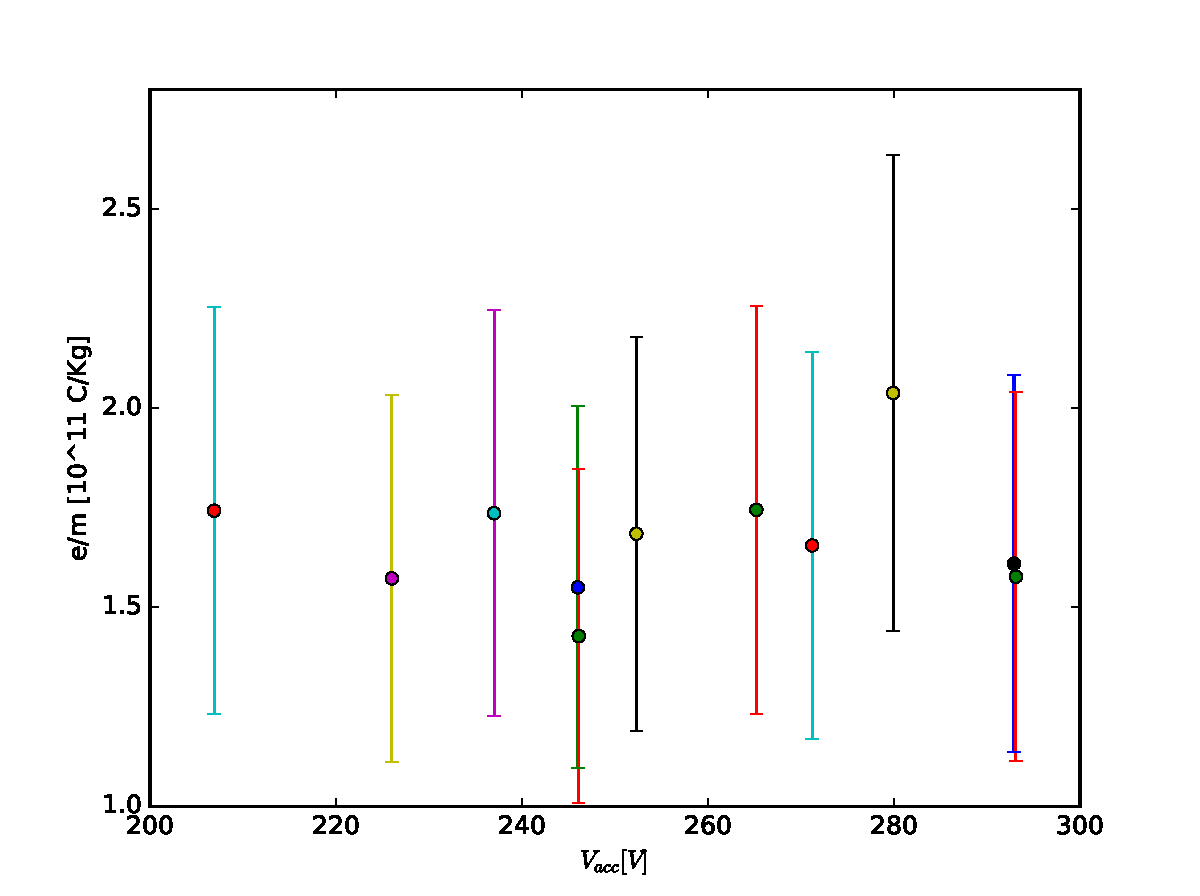
\includegraphics[scale=0.6]{figura8.pdf}
	\caption{Andamento di e/m in funzione della tensione di accelerazione.}
	\label{f:figura_8}
\end{figure}
\begin{figure}[h]
	\centering
	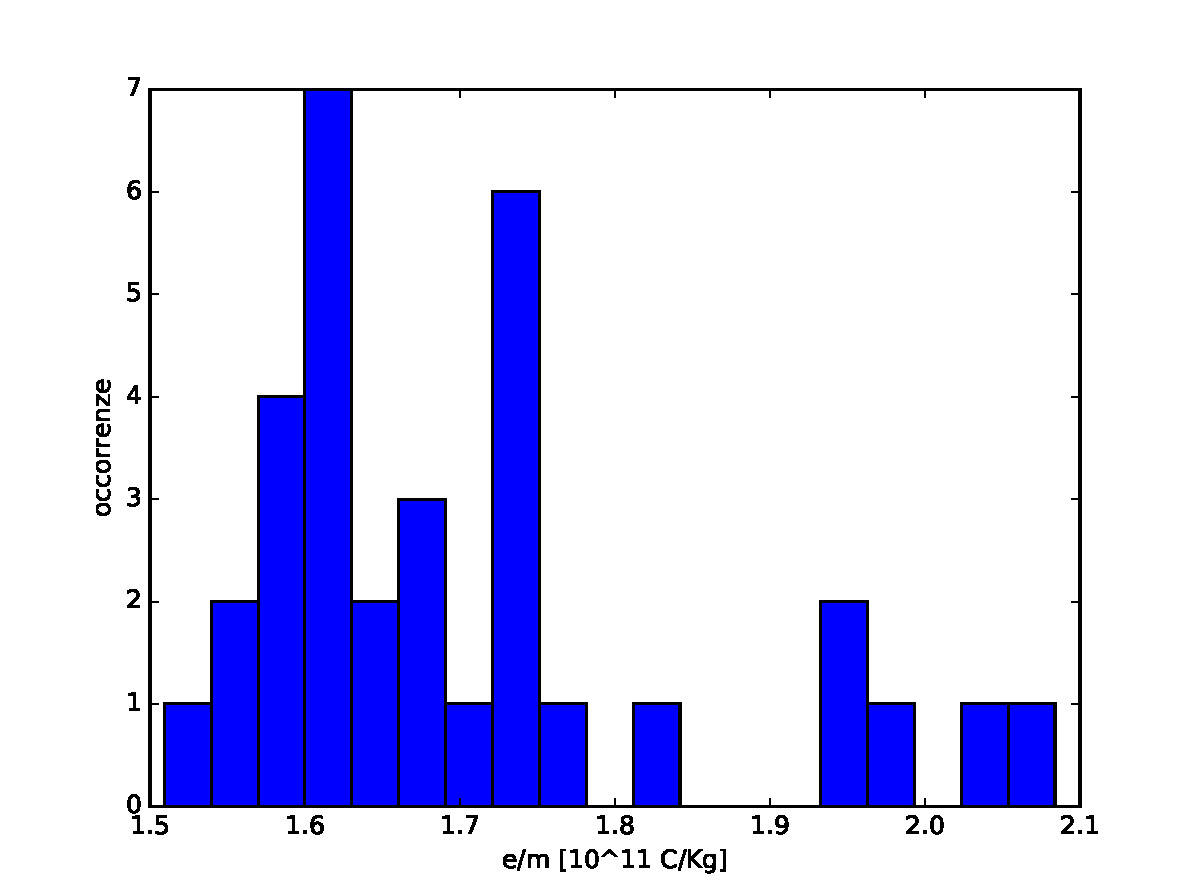
\includegraphics[scale=0.7]{figura9.pdf}
	\caption{istogramma per e/m}
           \label{f:figura_9}
\end{figure}
\begin{figure}[h]
	\centering
	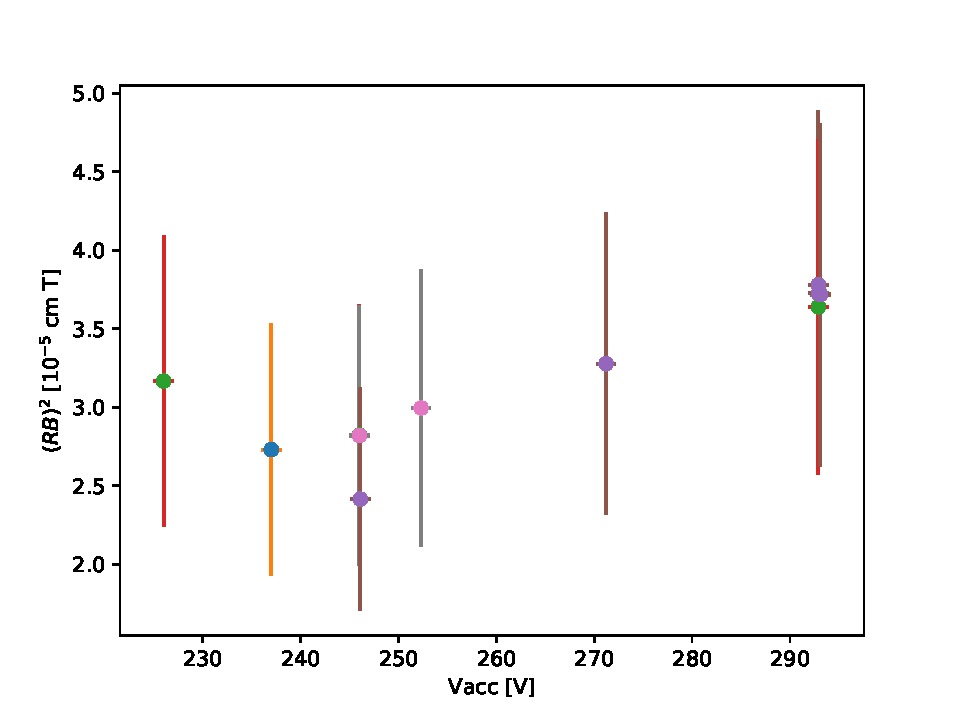
\includegraphics[scale=0.7]{figura10.pdf}
	\caption{${B_z r}^2$ in funzione di V$_{acc}$ con relativi residui.}
           \label{f:figura_10}
\end{figure}






